\documentclass[12pt]{article}
%Gummi|065|=)

\title{\textbf{
caracteristicas de los convertidores de potencia}}
\author{Guzman Vazquez Jaime Alan Yamil}
\date{19-sep-19}
\usepackage{graphicx}
\begin{document}

\begin{figure}[htp]
\centering

\includegraphics[scale=1.00]{/home/emile/Escritorio/reporte 1/índice.png}
\caption{}
\label{}
\end{figure}
\title
\SECTION {REPORTE DE PRACTICA\\CIRCUITOS DE RECTIFICACION NO CONTROLADOS\\\\Guzman Vazquez Jaime Alan Yamil\\
Rodriguez Lopez Francisco Javier\\ \\Sistemas electronicos de interfaz\\\\ }


\title
\section{Introduccion}
\\En este reporte se abundara en todas las cuestiones que se refieren a la practica que se realizo en la semana anterior, la practica consistia en generar las señales de diferentes partes en diferentes esquematicos , ejemplificando esto tenemos la señal de un duplicador de tension que como lo dicta su nombre duplica la tension de la salida de una señal, estos cinco circuitos fueron realizados en el software de diseño de circuitos profesional ORCAD que es un software de grado industrial diseñado para generar cualquier tipo de simulacion por medio del simulador llamado PSPICE que te permite controlar y manipular diferentes señales asi com ampliarlas o minimizarlas para conseguir los graficos necesarios para  la practica\\
Asi pues explicaremos todo el contexto de estos circuitos  y sus diferentes aspectos asi como el uso que se les da en la industria, esto sera explicado en el marco teorico en donde abundaremos en estas cuestiones, a continuacion se explicara el desarrollo de la practica en donde se expliicaran los paso que se siguieron en esta a continuacion y ya esxplicada la misma se procedera a dar la conclusiones de cada uno de los colaboradores de forma independiente, esta sera la manera que se realizara este documento.\\\\\\
\title
\section{Marco teorico}
\\En este apartado explicaremos los circuitos que se nos presentan y una introduccion y contexto a estos temas.\\

TIPOS DE RECTIFICADORES
\\Para mantener un voltaje continuo se rectifica un conjunto de voltajes alternos senoidales que forman un sistema polifasico equilibrado, estos voltajes son suministrados por una red monofasica o trifasica atravez de un transformador, cuyas misiones son:\\
\\*Ailsar galvanicamente la salida de corriente continua del generador de alterna .
\\*Acomodar el valor del voltaje de salida gracias a la relacion de transformacion.
\\*mediante una configuuracion adecuada , contribuir a disminuir el rizado a la salida.
\\estas son las clasificaciones que tienen:\\\\
*rectificacion en tipo paralelo(P) o de media onda :\\ las fases estan conectadas en estrella los devanados secundarios, cada uno en serie con su diodo estan montados en paralelo entre los bornes de salida.
\\*rectificador tipo paralelo doble(PD)\\\\
los devenados estan tambien conectados en estrella pero utlizando diodos por tanto estan formados por dos conmutadores de diodos cada uno, uno con catodos unidos y el otro con anodos unidos .\\\\
*rectificador de tipo serie (S):
\\dons devanados donde aparecen las tensiones alternas se conectan en poligono la suma de tensiones en esta configuracion es nula, existen dos diodos  agrupados  en dos conmutadores de diodos cada uno, unos con catodos unidos y el otro con anodos unidos .\\\\

 \begin{figure}[htp]
\centering
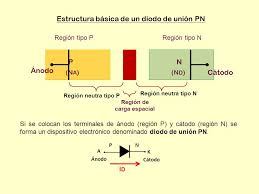
\includegraphics[scale=1.0]{/home/emile/Escritorio/reporte 1/tipo p.jpeg}
\caption{rectificacion tipo p}
\label{rectificacion tipo p }
\end{figure}
\begin{figure}[htp]
\centering
\includegraphics[scale=1.0]{/home/emile/Escritorio/reporte 1/índtipo pd.png}
\caption{rectificador PD}
\label{rectificador PD}
\end{figure}
\begin{figure}[htp]
\centering
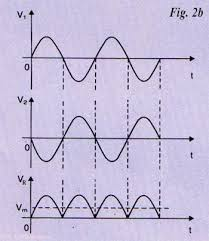
\includegraphics[scale=1.0]{/home/emile/Escritorio/reporte 1/images.jpeg}
\caption{rectificador tipo s }
\label{rectificador tipo s}
\end{figure}.
 
   
   
   
   
   
    
\title 
\section{Estas imagenes representas las ondas o los diagramas de dichas figuras.}\\\\

\title
\section{materiales}



















\title
\section{desarrollo:}
\\En breve explicaremos la practica que fue realizada primero explicaremos los pasos que seguimos para despues mostrar imagenes del contenido.\\
para esta practica lo primero que se debe hacer por mas intuitivo que parezca es instalar el software de diseño ORCAD al igual que todos sus complementos, teniendo todos los programas necesarios se procedio a realizar los esquematicos de cada uno de los diagramas que se nos presentaron en la practica, cuidando los aspectos como las fuentes de corriente alterna correspondiera al modelo de symbolo que ORCAD tiene especializado para  generar las señales en PSPICE y que no resultaran señales continuas o  compatibles, al igual que esto se tiene que verificar todos los componentes debido a que ORCAD cuenta con varias distribuciones de librerias diferentes que hacen distintas maneras de maipulacion al momento de ser simuladas por esto se tienen que buscar las que sean analogas buscando la mayor exactitud de estas.\\
Despues de concluir y tener todos los esquemaicos de todos los circuitos se procedio a generar las distintas simulaciones abriendo un nuevo perfil de simulacion y incluyenndo en ella las caracteristicas de esta como lo podrian ser el tiempo de inicio, el progreso en el tiempo que contiene las simulacion, etc . esto siempre orientado a el analisis conforme al tiempo ya que este software puede analizar en distintos rubros como lo puede ser el ruido de las señales, etc.\\
al terminar la  configuracion de la simulacion y los esquemmaticos, se procedio a colocar las puntas de en la parte que la practica dictaba que se tendria que dar por ejemplo a la salida de un capacitor etc, despues de colocar todas las puntas se procede a correr la simulacion y elegir que tipo de variable se quiere analizar como lo seria el analizis del voltaje de entrada, el analisis del voltaje de salida, en cada nodo, en alguno de los diodos y este software de diseño te graficara el mismo mostrandote el comportamiento de las ondas y sus deformaciones en funcion de los componentes incluidos en este.\\
basicamente esas fuero las cuestiones que se trataron en esta practica, adicionalmente se creo el PCB en el software de diseño  KICAD por ser mas intuitivo y mas rapido de usar, los PCB fueron creados a partir de exportar las huellas de los componentes la placa del PCB y despues cercar el mismo y agregar la conexion a tierra.\\\\
A continuacion veremos algunas imagenes de los esquemas asi como de las simulaciones.\\\\

\begin{figure}[htp]
\centering
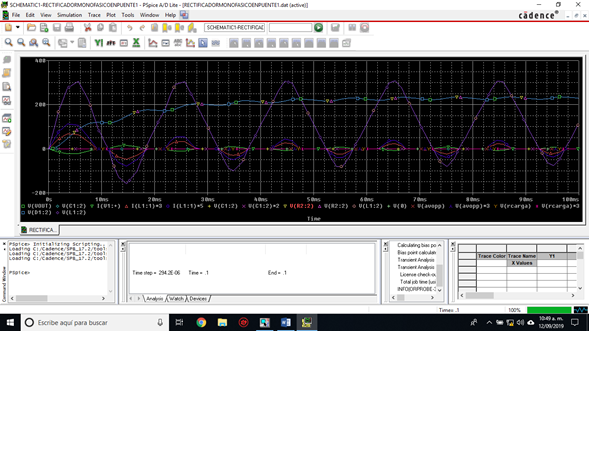
\includegraphics[scale=0.50]{monofasico1.png}
\caption{circuito monofasico}
\label{}
\end{figure}


\begin{figure}[htp]
\centering
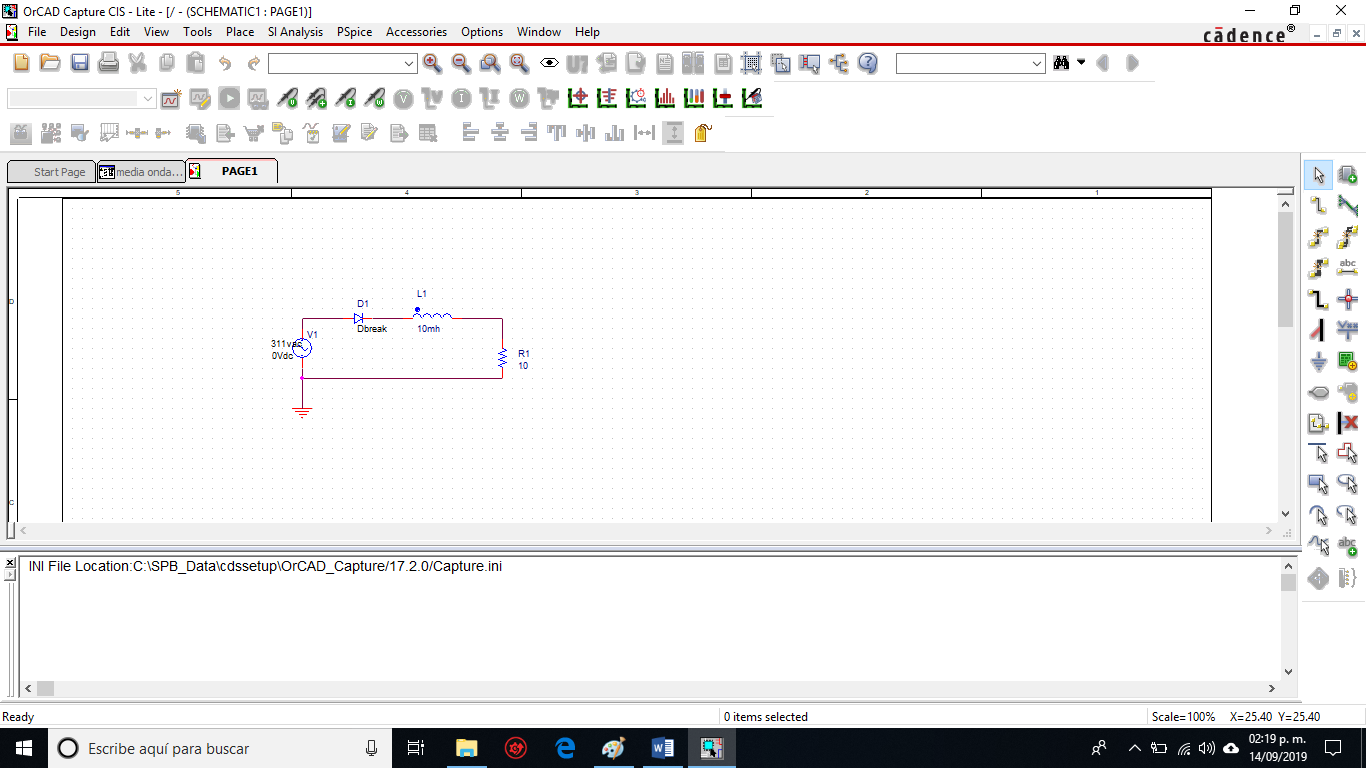
\includegraphics[scale=0.30]{esquema monofasico1.png}
\caption{monofasico esquematico}
\label{monofasico esquematico}
\end{figure}

\begin{figure}[htp]
\centering
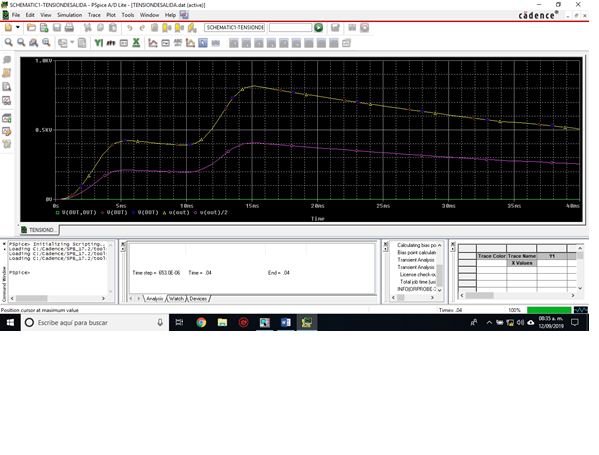
\includegraphics[scale=0.70]{duplicador de tension , salida de los condensadores.png}
\caption{duplicador de tension}
\label{duplicador de tension}
\end{figure}





\title
\section{Conclusion:Jaime Guzman}
\\En esta practica aprendimos a utilizar el software de ORCAD para realizar las simulaciones correspondientes en los diferentes circuitos, esto de mi parte fue algo nuevo ya que nunca habia utilizado este software de diseño sin embargo cumplio las espectativas que se tenian de el, los esquematicos cada uno cumple una funcion especifica o contiene un tipo de diferente de caracteristica que lo diferencia de los demas, algunos tenian tres fuente de corriente otros tenian un puente de diodos adjuntado a una bobina o capacitores y cada configuracion realiza alguna funcion , algus amplifican la señal de entrada en la salida y algunos otros retrasan la señal formando un pico desfasado o una onda desfasada, algunos otros rectifican la onda completa generando de una corriente alterna a una practicamente directa o incluso algunos otros rectifican solamente la mitad de la onda estos diferentes aspectos de cada circuito, el realizarlos en pcb  al igual que en esquematico y cada una de sus ondas fue muy interesante ademas de ayudar mucho a la formacion de los alumnos en cuanto a la electronica de potencia ademas de el software de diseño de circuitos.

\title
\section{Conclusion: Francisco Rodriguez}
\\



\end{document}